%%%%%%%%%%%%%%%%%%%%%%%%%%%%%%%%%%%%%%%%%%%%%%%%%%%%%%%%%%
% Ping GCM
%%%%%%%%%%%%%%%%%%%%%%%%%%%%%%%%%%%%%%%%%%%%%%%%%%%%%%%%%%
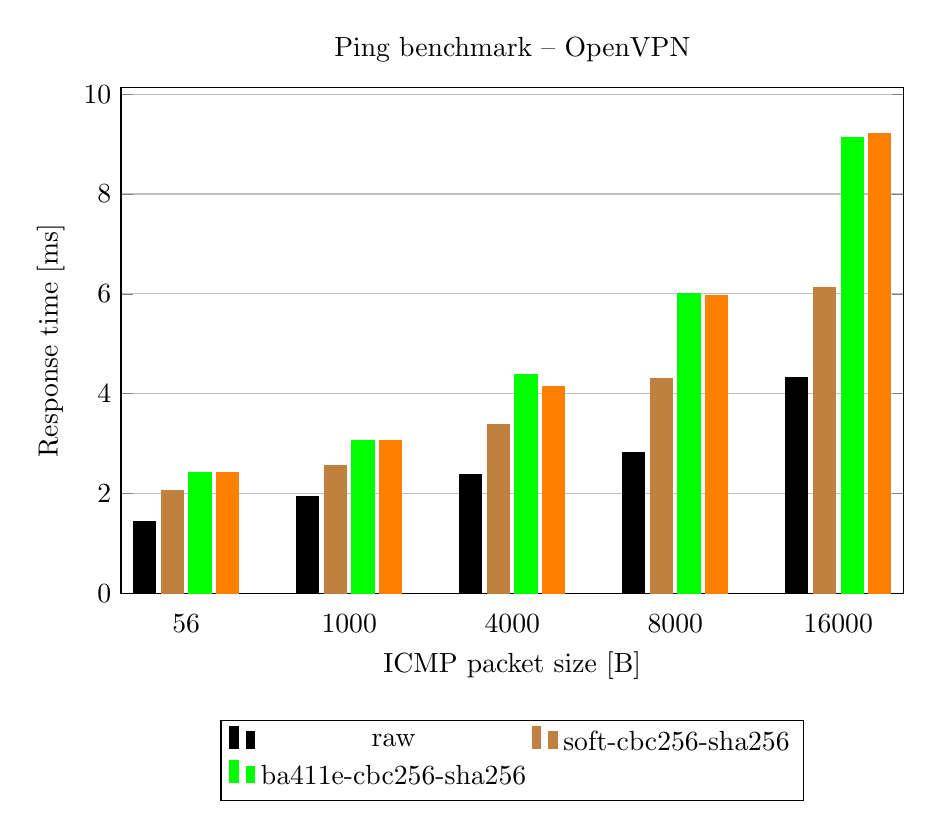
\begin{tikzpicture}
\begin{axis}[
        title = {Ping benchmark -- OpenVPN},
        width  = 0.95*\textwidth,
        height = 8cm,
        major x tick style = transparent,
        ybar,
        bar width=8pt,
        ymajorgrids = true,
        ylabel = {Response time [ms]},
        xlabel = {ICMP packet size [B]},
        ymin=0,
        symbolic x coords={56, 1000, 4000, 8000, 16000},
        xtick = data,
        scaled y ticks = false,%Disable the *10^4 exponent applied to all y axis markings.
        legend style={at={(0.5,-0.25)}, anchor=north,legend columns=2},
        enlarge x limits=0.1,
    ]
% I would have prefered to have "\addplot[marks only]", but they overlap if they have the same x coordinate,
% not like bars that automatically shift.
\addplot[style={black, fill=black}]
    coordinates {
        (56, 1.444)
        (1000, 1.929)
        (4000, 2.376)
        (8000, 2.811)
        (16000, 4.322)
    };
    \label{raw}

\addplot[style={brown, fill=brown}]
    coordinates {
        (56, 2.066)
        (1000, 2.561)
        (4000, 3.373)
        (8000, 4.293)
        (16000, 6.117)
    };
    \label{none-none}

\addplot[style={green, fill=green}]
    coordinates {
        (56, 2.415)
        (1000, 3.061)
        (4000, 4.376)
        (8000, 5.997)
        (16000, 9.135)
    };
    \label{soft-cbc256-sha256}

\addplot[style={orange, fill=orange}]
    coordinates {
        (56, 2.416)
        (1000, 3.052)
        (4000, 4.140)
        (8000, 5.963)
        (16000, 9.207)
    };
    \label{ba411e-cbc256-sha256}

\legend{raw, soft-cbc256-sha256, ba411e-cbc256-sha256}
\end{axis}
\end{tikzpicture}
% Here, I could show the gcm128, which show better performances with the BA411e, but I would be weird to compare it with aes256cbc.
% I need another graph with a CPu usage comparison to show that even if the perf are the same for soft/hard with aes256gcm, the hard loads less the CPU (I hope so, at least).